\documentclass{standalone}
\usepackage{color}
\usepackage{tikz}
\usetikzlibrary{shapes,arrows,arrows.meta,fit,positioning}

\newcommand{\defaultwidth}{6cm}
\tikzset{
    auto, node distance = 2cm,
    stage/.style = { draw, thick, rectangle, align=center,
        text width = \defaultwidth, 
        font=\bfseries,
        rounded corners=2mm, 
        minimum width = \defaultwidth
    },
    note/.style = { draw, very thin, rectangle, dashed, align=center,
        node distance = 0.5cm,
        text width = \defaultwidth - 1cm, 
        font=\footnotesize,
        minimum width = \defaultwidth - 1cm
    },
    arrow/.style = { ->, very thick },
    arrow_text/.style = { align=center,
        pos = 0.5,
        text width = 3cm, 
        font = \scriptsize
    }
}

\begin{document}
    \begin{tikzpicture}
        \node[stage] (0) at (0,0)
            {Input \\ 
\includegraphics[width=\defaultwidth]{P1}};
        \node[scale=1.75] (A) at (0,-4) {a};
        \node[stage] (1) [right = of 0]
            {Partitioning \\ 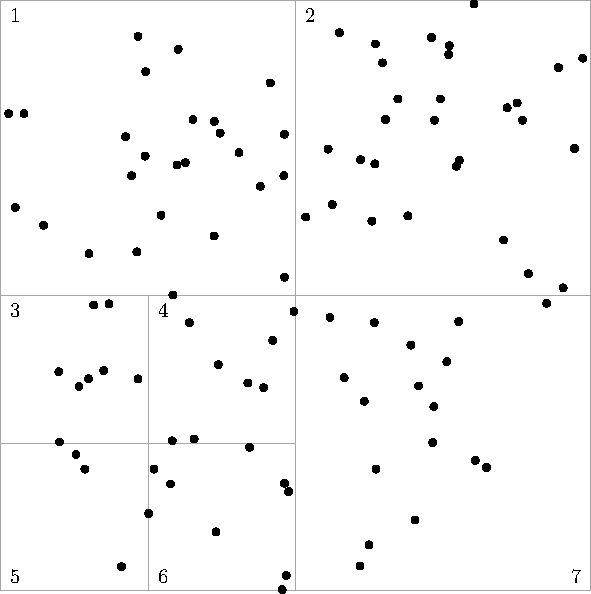
\includegraphics[width=\defaultwidth]{P2}};
        \node[scale=1.75] (A) at (8.5,-4) {b};
        \node[stage] (2) [right = of 1]
            {Replication \\ 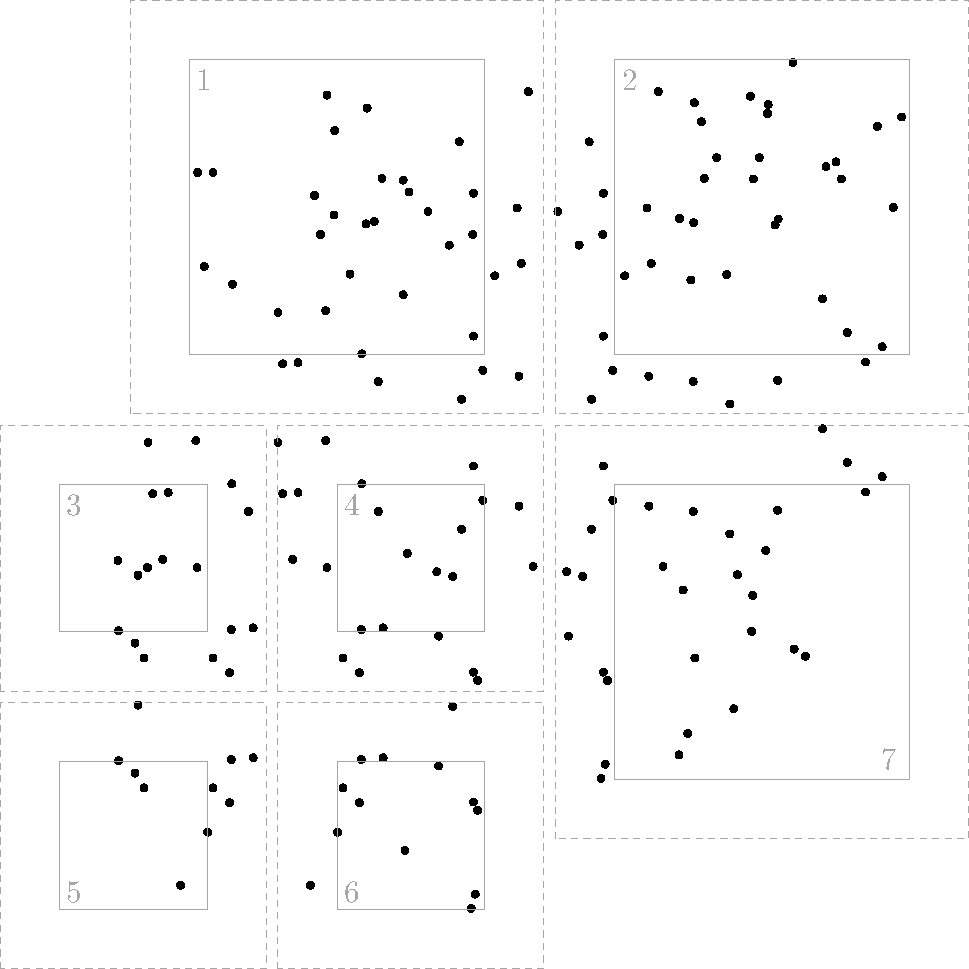
\includegraphics[width=\defaultwidth]{P3}};
        \node[scale=1.75] (A) at (17,-4) {c};
        \draw[arrow] (0) --  (1);
        \draw[arrow] (1) --  (2);
    \end{tikzpicture}
\end{document}
